% Copyright 2004 by Till Tantau <tantau@users.sourceforge.net>.
%
% In principle, this file can be redistributed and/or modified under
% the terms of the GNU Public License, version 2.
%
% However, this file is supposed to be a template to be modified
% for your own needs. For this reason, if you use this file as a
% template and not specifically distribute it as part of a another
% package/program, I grant the extra permission to freely copy and
% modify this file as you see fit and even to delete this copyright
% notice. 


\documentclass[9pt]{beamer}
\usepackage{graphicx}                       % loads images
\usepackage{color}                          % for color in text
\usepackage{float}                          % to place [H]
\usepackage{amsmath}
\usepackage{amssymb}
\usepackage{bbm}
\usepackage{booktabs}
\usepackage{longtable}
\usepackage{bigstrut}
\usepackage{array}
    
\usepackage{multirow}
\usepackage{xr}
\usepackage[round]{natbib}


%  \usepackage[backend=biber, style=alphabetic ,
% citepstyle=authoryear]{biblatex}[2016/01/01] %the latest version of biblatex?
  % biber is version 2.4; the latest?
%\addbibresource{References.bib}




\graphicspath{{./Figuras/}}
\usepackage{color}
%\usepackage{morefloats}
%\usepackage{showkeys}

\usepackage{enumerate}
\usepackage[labelfont=bf]{caption}
\usepackage[labelfont=bf, justification=justified]{subcaption}
\captionsetup{position=top}
\captionsetup[subfigure]{justification=centering}



\usepackage{epstopdf}
\epstopdfDeclareGraphicsRule{.tiff}{png}{.png}{convert #1 \OutputFile}
\AppendGraphicsExtensions{.tiff}


\usepackage{setspace}

\renewcommand{\rmdefault}{ppl}
\definecolor{darkred}{rgb}{0.8, 0.0, 0.0}
\definecolor{navyblue}{rgb}{0.0, 0.0, 0.8}
\definecolor{cadmiumgreen}{rgb}{0.0, 0.6, 0.24}

\usepackage{hyperref}
\hypersetup{
    pdfstartview={FitH},    		% fits the width of the page to the window
    pdftitle={Overconfidence and settlement: evidence from Mexican Labour courts},    % title
    pdfauthor={CJMS},     % author
    colorlinks=true,       % false: boxed links; true: colored links
    linkcolor=white,          % color of internal links (change box color with linkbordercolor)
    citecolor=darkred,        % color of links to bibliography
    filecolor=magenta,      % color of file links
    urlcolor=darkred           % color of external links
}

\newcommand{\green}[1]{\textcolor{cadmiumgreen}{#1}}

\newcommand{\comment}[1]
{\par {\bfseries \color{blue} #1 \par}}
%\usepackage{showkeys}


% There are many different themes available for Beamer. A comprehensive
% list with examples is given here:
% http://deic.uab.es/~iblanes/beamer_gallery/index_by_theme.html
% You can uncomment the themes below if you would like to use a different
% one:
%\usetheme{AnnArbor}
%\usetheme{Antibes}
%\usetheme{Bergen}
%\usetheme{Berkeley}
%\usetheme{Berlin}
%\usetheme{Boadilla}
%\usetheme{boxes}
%\usetheme{CambridgeUS}
%\usetheme{Copenhagen}
%\usetheme{Darmstadt}
%\usetheme{default}
%\usetheme{Frankfurt}
%\usetheme{Goettingen}
%\usetheme{Hannover}
%\usetheme{Ilmenau}
%\usetheme{JuanLesPins}
%\usetheme{Luebeck}
\usetheme{Madrid}
%\usetheme{Malmoe}
%\usetheme{Marburg}
%\usetheme{Montpellier}
%\usetheme{PaloAlto}
%\usetheme{Pittsburgh}
%\usetheme{Rochester}
%\usetheme{Singapore}
%\usetheme{Szeged}
%\usetheme{Warsaw}

\setbeamertemplate{headline}{%
    \leavevmode%
    \hbox{%
        \begin{beamercolorbox}[wd=\paperwidth,ht=2.5ex,dp=1.125ex]{palette quaternary}%
            \insertsectionnavigationhorizontal{\paperwidth}{}{\hskip0pt plus1filll}
        \end{beamercolorbox}%
    }
}

\title{Statistical information and settlement}

% A subtitle is optional and this may be deleted
\subtitle{Evidence from Mexican labor courts}

\author{J. Sadka\inst{1} \and E. Seira\inst{2} \and C. Woodruff\inst{3}}
% - Give the names in the same order as the appear in the paper.
% - Use the \inst{?} command only if the authors have different
%   affiliation.

\institute[ITAM, Oxford] % (optional, but mostly needed)
{
  \inst{1,2}%
  ITAM
  \and
  \inst{3}%
  Oxford
}
% - Use the \inst command only if there are several affiliations.
% - Keep it simple, no one is interested in your street address.

\date{IEA, 2017}
% - Either use conference name or its abbreviation.
% - Not really informative to the audience, more for people (including
%   yourself) who are reading the slides online

\subject{Applied Microeconomics}
% This is only inserted into the PDF information catalog. Can be left
% out. 

% If you have a file called "university-logo-filename.xxx", where xxx
% is a graphic format that can be processed by latex or pdflatex,
% resp., then you can add a logo as follows:

% \pgfdeclareimage[height=0.5cm]{university-logo}{university-logo-filename}
% \logo{\pgfuseimage{university-logo}}

% Delete this, if you do not want the table of contents to pop up at
% the beginning of each subsection:

% Let's get started
\begin{document}

\begin{frame}
  \titlepage
\end{frame}

\begin{frame}{Outline}
  \begin{enumerate}
      \item Motivation and literature
      \item Context
      \item Anecdotal story
      \item Diagnostic data
      \item Experiment and results
      \item Work in progress
  \end{enumerate}
\end{frame}



\section{Motivation}

\begin{frame}{Motivation}{}
  \begin{itemize}
  \item {Courts function poorly in most developing countries: backlogs, delay, unpredictable case outcomes. This hampers the functioning of markets and raises concerns for access to justice.}
  \vspace{.1in}
  \item {Little rigorous evidence on the ineffectiveness of courts and its causes.}
  \vspace{.1in}
  \item{Recently Mexico pushed a \alert{reform that moves labor lawsuits to judicial branches and creates a pre-lawsuit compulsory conciliation stage}...still in design.}
  \vspace{.05in}
    \begin{itemize}
        \item Can institutional pre-conciliation stage increase settlement?
          \vspace{.05in}
        \item Can statistical information increase settlement?
    \end{itemize}
    \vspace{.1in}
    \item {This presentation:}
       \begin{itemize}
           \item First document some \alert{stylized facts} about settlement and misinformation in a Mexican labor court.
           \item Then show the results of an \alert{experiment} aimed at increasing the information available to parties who then decide whether to settle or continue a lawsuit.
       \end{itemize}
  \end{itemize}
\end{frame}
                  

\begin{frame}{Related Literature}
\begin{itemize}
    \item Effects of Labor laws: \citep{Botero_Regulation},  \citep{PonticelliAlencar_Bankrupcy}.
    \vspace{.1in}
    \item Bargaining and delay in litigation. 
        \begin{itemize}
        \item Informational asymmetries: credibly communicate private value through (inefficient) waiting \citep{Cramton_1991, Cramton_1992}, \citep{Cramton_1994a, Cramton_1994b}
        \item Overconfidence: \citep{Yildiz_CommonPrior}, \citep{Farber_DivergentExpectations}
        \item Behavioral biases: \citep{BabcockLoewensein_BargainingImpasse}, \citep{camerer_behavioral}.
    \end{itemize}
    \vspace{.1in}
    \item Lab experiments with bargaining and litigation settings: \citep{Ashenfelter_DisputeRates}, \citep{Pogarsky_DamageCaps}, and  \citep{Sullivan_Experimental}.
    \vspace{.1in}
    \item We know of no field experiment conducted in labor courts studying the decision of parties to settle.
\end{itemize}
\end{frame}


\section{Context}

\begin{frame}{Context}
   \begin{itemize}

       \item \textbf{The lawsuits:} We deal with firing disputes, courts must determine fair/unfair dismissal. 
       \vspace{0.05in}
         
        \item \textbf{The law:} Proving fair dismissal is difficult; legal severance is a minimum of three months' wage with benefits.  
        \vspace{0.05in}
         
        \item \textbf{The court:} We work with the Mexico City Labor Court (MCLC).
        \vspace{0.05in}
        \begin{itemize}
            \item Largest local labor court in Latin America (receives 30,000 new cases per year).
            \item Its backlog would take 4 years to process.
        \end{itemize}
                                
       %\item \textbf{Conciliation mandated by law:} The first hearing is supposedly dedicated to "conciliation". The MCLC has 1 assigned conciliator per individual court.
       %\vspace{0.05in}
       
       \item \textbf{What happens if they don't settle:} Defendant answers, evidence is submitted and viewed, and the court issues a judgment.
       \vspace{0.05in}
       
       \item \textbf{Enforcement:} is not trivial. Between 30 and 50 percent of decisions favorable to the worker will end up being unenforceable. 
       
       \end{itemize}         
        
     \end{frame}
     
     
\begin{frame}{... More context}
    \begin{itemize}     
       \item \textbf{Lawyers:} Legal representation is necessary to file a lawsuit. Lawyers dominate the process of the lawsuit. The presence of the parties themselves at the hearings is not compulsory. 
       \vspace{0.05in}
       
        \item   \textbf{Workers:} can hire private lawyers or a free lawyer from the public labor prosecutor's office.
        \vspace{0.05in}
            \begin{itemize}
                \item Public lawyers:
                \begin{itemize}
                    \item Paid a flat wage and cannot charge additional fees.
                    \item Generally well qualified, but overworked: they handle 10 times more cases on average.
                \end{itemize}
                \vspace{0.05in}
                \item Private lawyers:
                \begin{itemize}
                    \item They must be licensed, but do not have to pass a bar exam.
                    \item Charges: initial fee to file the lawsuit (around 150 USD), contingency fee of 30-40 percent.
                    \item Large variation in quality (anecdotal evidence).
                \end{itemize} 
            \end{itemize}

    \end{itemize}
\end{frame}


\begin{frame}{Anecdotal Story}
\textbf{Moral hazard by private lawyers:} Private lawyers have more information than workers and convince them to sue by inflating their expectations of winning. Two main drivers:
\vspace{0.1in}
    \begin{itemize}
        \item \textbf{Low information environment}: Suing workers have:
        \begin{itemize}
            \item Little information of the law
            \item No repeated experience
            \item Propensity to biased expectations (selection, angry)
        \end{itemize}
        \vspace{0.1in}
        \item \textbf{Incentives of Private Lawyers:} Inflating the claim and not settling. Why?
        \begin{itemize}
                \item Less risk averse than the worker as they handle many cases
                \item They make a profit from just filing 
                %\item Even bad lawyers have some low probability of winning, due to excessive formalism, the low quality of the labor courts, and corruption. ESTO LO QUITE PORQUE AQUI SI ESTA ALINEADO CON EL WORKER
         \end{itemize}
          \vspace{0.1in}
        \item{While our data shows low-information of workers and inflated initial claim of private lawyers, we have not yet nailed the moral hazard story} 
            \begin{itemize}
                \item The main problem is that lawyers selection is endogenous to claims, misinformation, etc.
            \end{itemize}
    \end{itemize}
\end{frame}



\section{Data}

\begin{frame}{Data}{}
   \begin{itemize}
       \item \textbf{Partner:} Mexico City Labor Court (individual court 7).
       \vspace{0.1in}

        \item \textbf{Historical Data:} Use it for diagnostics and \alert{``Calculator prediction''}.
        \vspace{0.05in}
            \begin{itemize}
                \item \textbf{Sample:} 2500 \textit{concluded} cases from subcourt 7. Random sample of all cases filed in 2011 and 2012 which were concluded by the end of 2015.
                \vspace{0.05in}
                    \begin{itemize}
                        \item Currently evauating this selection problem.
                    \end{itemize}
                \item \textbf{Variables:} Initial labor suit variables (e.g. wage, tenure); When the suit ended and how (settlement, drop, judgment, or expiry); compensation received by the worker.
            \end{itemize}
            \vspace{0.1in}
        \item \textbf{Survey pilot data:} 70\% of cases with notified hearings conducted between March and May 2016: 1103 casefiles.
        \vspace{0.05in}
            \begin{itemize}
                \item \textbf{Parties:} Lawyers almost always present, worker present $\leq$ 20\% of the time. 
                \vspace{0.05in}
                \item \textbf{Baseline survey}: education, how they found their lawyer, payment to lawyer, expectations about win probability and amount, lawsuit duration, knowledge of the law and of own claims.
                \vspace{0.05in}
                \item \textbf{Exit survey}: expectations after trial (only for people who did not settle unfortunately). About 50\% take up.
            \end{itemize}
   \end{itemize}
\end{frame}


\section{Stylized Facts}

\begin{frame}{Stylized Facts: Long Duration}
    \begin{itemize}
        \item \textbf{Fact 1 (Low settlement rates in spite of long trials):}
            \begin{itemize}
            \vspace{0.05in}
                \item Mexico 52\% of cases are settled.
                \vspace{0.05in}
                \item  Even those who settle take a long time to do so.
                \vspace{0.05in}
                \item 79\% in Australia, 80\% US, 90\% Sweden.
            \end{itemize}
    \end{itemize}
    \begin{figure}[H]
    \label{DurationFig}
    \begin{center}
        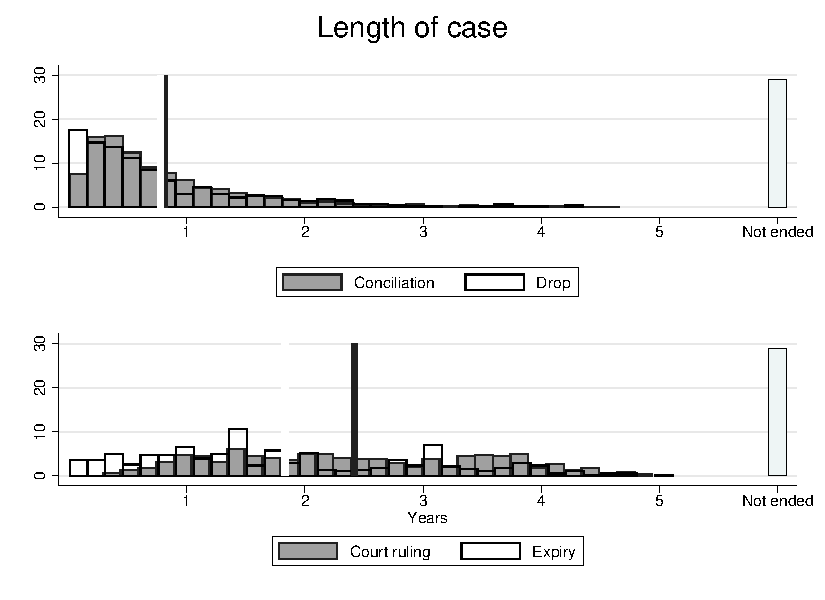
\includegraphics[width=0.6\textwidth]{Duracion.pdf}
        \end{center}
\end{figure}
\end{frame}


\begin{frame}{Stylized Facts: Recovery is low}
    \begin{itemize}
        \item \textbf{Fact 2 (Awards are low):} The amount awarded is a small percentage of the amount asked for, and is even less than what the law mandates.
            
    \end{itemize}
    \begin{figure}[H]
    \label{claimsvsoutcomes}
    \begin{center}
        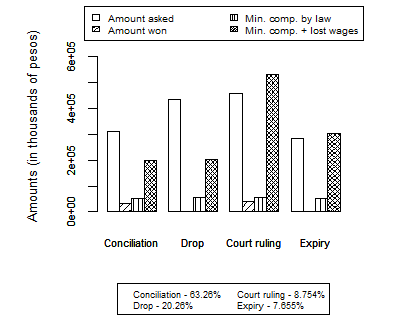
\includegraphics[width=0.6\textwidth]{Amountasked.tiff}
        \end{center}
    \end{figure}    
\end{frame}



\begin{frame}{Stylized Facts: Misinformation}
    \begin{itemize}
        \item \textbf{Fact 3 (Misinformation):}
        \vspace{0.05in}
        \begin{itemize}
            \item Only 60\%  know what they are claiming overtime in their own lawsuit. 
            \vspace{0.05in}
            \item Only one-third of workers know what the legal severance pay is.
        \end{itemize}
        
    \end{itemize}
    
       \begin{figure}[H]
    \begin{center}
        \begin{subfigure}{0.49\textwidth}
            \caption{Overtime}
            \centering
            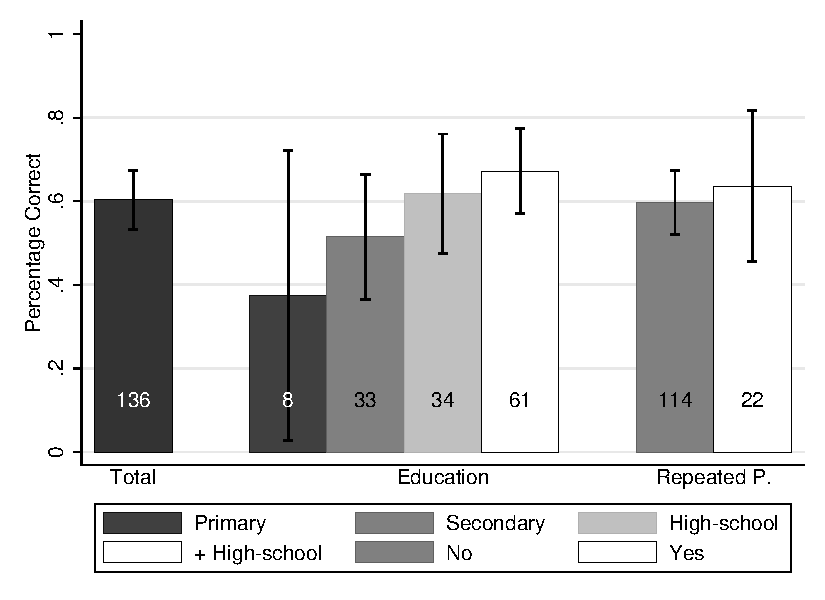
\includegraphics[width=1\textwidth]{Extra_hrs.pdf}
        \end{subfigure}
        \begin{subfigure}{0.49\textwidth}
            \caption{Severance}
                \centering
                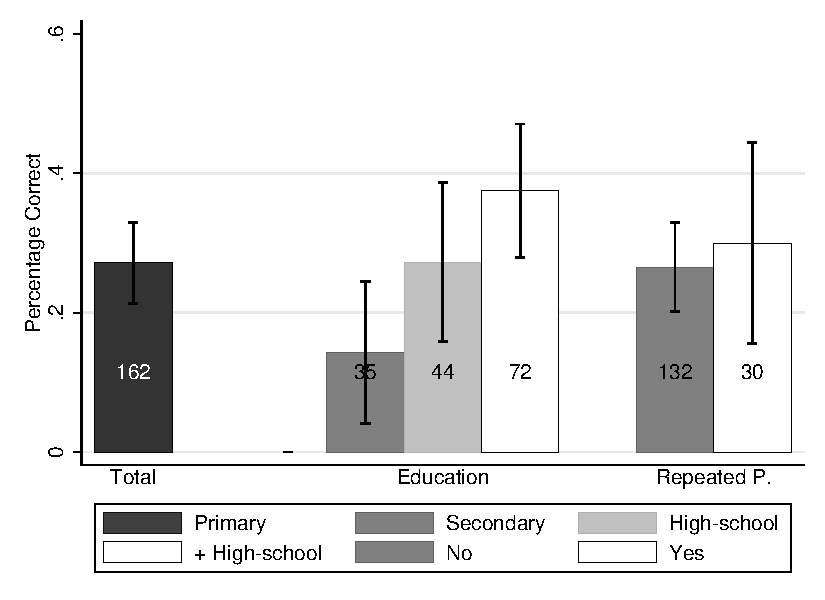
\includegraphics[width=1\textwidth]{Correctly_knows.pdf}
        \end{subfigure}
        \end{center}
\end{figure}

   
\end{frame}




\begin{frame}{Inflated expectations}
    \begin{itemize}
        \item  \textbf{Fact 4 (Overconfidence):} Plaintiffs on average think they will win 78\% of the time, while their average win rate in the data is 41\%. The sum of subjective probabilities of winning for the same cases is 1.47.
        \vspace{0.2in}
        
         \item \textbf{Fact 5 (Inflated claim and not more money awarded):} Controlling for observables, private lawyers ask for 137,592 pesos more than public lawyers, and only get 10,531 pesos more in settlements.
    \end{itemize}
  
\end{frame}


\section{Experiment and Results}

\begin{frame}{Experiment: provide information to debias parties}

    Given the environment of low information, misaligned incentives, overconfidence, and the possibility of private lawyer moral hazard...
        \vspace{0.1in}
        
    \begin{itemize}
        \item \textbf{Treatment 1: ``Calculator''.} provide (objective) statistical information that could help ''debias'' the plaintiff's expectations and lead to more settlement.
          \begin{itemize}
              \item Probability and amount won conditional on winning
              \item Unbiased prediction (out of sample tests -- good fit)
              \item Explained that is was an average for concluded cases similar to theirs.
          \end{itemize}
        \vspace{0.1in}
        \item \textbf{Treatment 2: ``Expert advice''.} Face-to-face advice from a conciliator.
        \vspace{0.1in}
        \item{\textbf{Outcomes:} settlement, expectation updating}
         \vspace{0.1in}
        \item \textbf{Welfare:} we will not make welfare claims, but...
            \begin{itemize}
                \item The law encourages settlement.
                \item In (most?) models of bargaining with asymmetric information welfare increases as information is less asymmetric and more precise.
            \end{itemize}
    \end{itemize}
\end{frame}




\begin{frame}{Experiment flowchart}
\begin{columns}[T]
    \begin{column}{.6\textwidth}
    \begin{itemize}
        \vspace{.2in}
        \item The experiment started on March 2, 2016 and ended on May 27, 2016.
        \item 1103 casefiles intervened before hearing.
        \vspace{0.1in}
        \item We randomized into 3 arms (control, calculator, conciliator) with equal probabilities. 
            \begin{itemize}
                \item Balance tests passed in assignment and take-up sample.
            \end{itemize}
        \vspace{0.1in}    
        \item Take up of the treatment was about 70\% in both arms. Take up exit survey 52\%.
       \end{itemize} 
    \end{column}
    \begin{column}{.5\textwidth}
    \begin{figure}[H]
   \label{treatment_flowchart}
    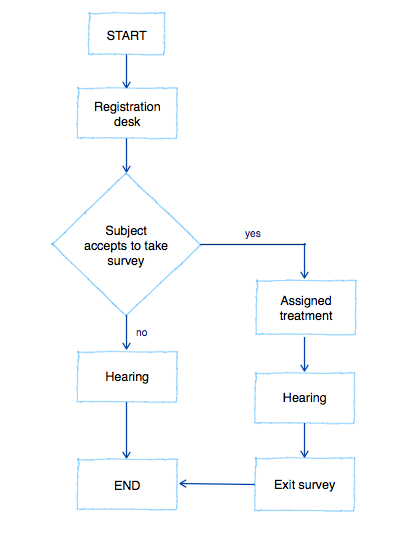
\includegraphics[width=0.8\textwidth]{./Figuras/Experiment_flowchart.png}
\end{figure}
\end{column}
  \end{columns}
\end{frame}




\begin{frame}{Calculator treatment}

    \begin{figure}[H]
    \label{calc_template}
    \begin{center}
        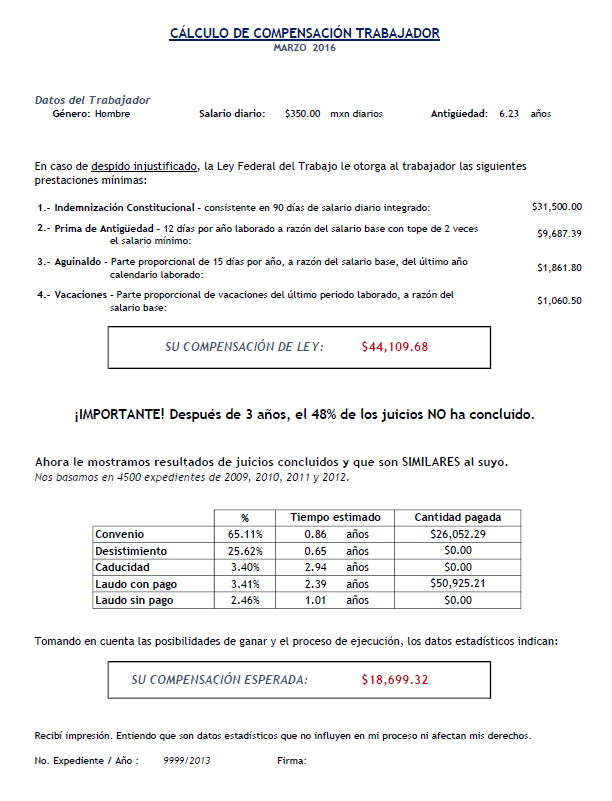
\includegraphics[width=0.55\textwidth]{calctreat.png}
        \end{center}
\end{figure}
\end{frame}




\begin{frame}{Main Result}
    \begin{itemize}
        \item We find that \textbf{\textit{same day} conciliation increases by 4pp} for calculator and conciliator, above the 5pp for control.
        \vspace{0.05in}
        \item The effect is \textbf{persistent 6 months later}, therefore not a ''lagged-communication'' story. 
        \vspace{0.05in}
        \item \textbf{Only when the worker present: 20pp effect then}.
    \end{itemize}
  \hskip-6.0cm\begin{table}
    \label{Table_effects_F}
    \tiny{% Table generated by Excel2LaTeX from sheet 'Minicortes_2'
\begin{tabular}{rrrrrrrrrr}
\toprule
      & \multicolumn{9}{c}{Panel A: Treatment on conciliation} \\
\midrule
      & \multicolumn{2}{c}{Same day} & \multicolumn{2}{c}{June} & \multicolumn{1}{c}{July } & \multicolumn{1}{c}{Aug} & \multicolumn{1}{c}{Sept} & \multicolumn{2}{c}{Oct} \\
      \midrule
\multicolumn{1}{l}{Control} & \multicolumn{1}{l}{0.0505***} & \multicolumn{1}{l}{0.0326***} & \multicolumn{1}{l}{0.0968***} & \multicolumn{1}{l}{0.0789***} & \multicolumn{1}{l}{0.116***} & \multicolumn{1}{l}{0.132***} & \multicolumn{1}{l}{0.169***} & \multicolumn{1}{l}{0.185***} & \multicolumn{1}{l}{0.171***} \\
\multicolumn{1}{l}{} & \multicolumn{1}{l}{(0.0113)} & \multicolumn{1}{l}{(0.0102)} & \multicolumn{1}{l}{(0.0153)} & \multicolumn{1}{l}{(0.0155)} & \multicolumn{1}{l}{(0.0166)} & \multicolumn{1}{l}{(0.0176)} & \multicolumn{1}{l}{(0.0195)} & \multicolumn{1}{l}{(0.0202)} & \multicolumn{1}{l}{(0.0217)} \\
\multicolumn{1}{l}{Calculator} & \multicolumn{1}{l}{0.0470**} & \multicolumn{1}{l}{0.0157} & \multicolumn{1}{l}{0.0497**} & \multicolumn{1}{l}{0.00847} & \multicolumn{1}{l}{0.0506*} & \multicolumn{1}{l}{0.0457*} & \multicolumn{1}{l}{0.0306} & \multicolumn{1}{l}{0.0455} & \multicolumn{1}{l}{0.00377} \\
\multicolumn{1}{l}{} & \multicolumn{1}{l}{(0.0193)} & \multicolumn{1}{l}{(0.0162)} & \multicolumn{1}{l}{(0.0243)} & \multicolumn{1}{l}{(0.0228)} & \multicolumn{1}{l}{(0.0258)} & \multicolumn{1}{l}{(0.0268)} & \multicolumn{1}{l}{(0.0288)} & \multicolumn{1}{l}{(0.0301)} & \multicolumn{1}{l}{(0.0312)} \\
\multicolumn{1}{l}{Conciliator} & \multicolumn{1}{l}{0.0419**} & \multicolumn{1}{l}{0.0152} & \multicolumn{1}{l}{0.0472**} & \multicolumn{1}{l}{0.0134} & \multicolumn{1}{l}{0.0475*} & \multicolumn{1}{l}{0.0503*} & \multicolumn{1}{l}{0.0372} & \multicolumn{1}{l}{0.0455} & \multicolumn{1}{l}{0.000922} \\
\multicolumn{1}{l}{} & \multicolumn{1}{l}{(0.0189)} & \multicolumn{1}{l}{(0.0158)} & \multicolumn{1}{l}{(0.0239)} & \multicolumn{1}{l}{(0.0226)} & \multicolumn{1}{l}{(0.0254)} & \multicolumn{1}{l}{(0.0267)} & \multicolumn{1}{l}{(0.0287)} & \multicolumn{1}{l}{(0.0299)} & \multicolumn{1}{l}{(0.0304)} \\
\multicolumn{1}{l}{Emp present (EP)} & \multicolumn{1}{l}{} & \multicolumn{1}{l}{0.0979**} & \multicolumn{1}{l}{} & \multicolumn{1}{l}{0.0975**} & \multicolumn{1}{l}{} & \multicolumn{1}{l}{} & \multicolumn{1}{l}{} & \multicolumn{1}{l}{} & \multicolumn{1}{l}{0.0789} \\
\multicolumn{1}{l}{} & \multicolumn{1}{l}{} & \multicolumn{1}{l}{(0.0419)} & \multicolumn{1}{l}{} & \multicolumn{1}{l}{(0.0489)} & \multicolumn{1}{l}{} & \multicolumn{1}{l}{} & \multicolumn{1}{l}{} & \multicolumn{1}{l}{} & \multicolumn{1}{l}{(0.0569)} \\
\multicolumn{1}{l}{Calculator\#\#EP} & \multicolumn{1}{l}{} & \multicolumn{1}{l}{0.158**} & \multicolumn{1}{l}{} & \multicolumn{1}{l}{0.206***} & \multicolumn{1}{l}{} & \multicolumn{1}{l}{} & \multicolumn{1}{l}{} & \multicolumn{1}{l}{} & \multicolumn{1}{l}{0.210**} \\
\multicolumn{1}{l}{} & \multicolumn{1}{l}{} & \multicolumn{1}{l}{(0.0707)} & \multicolumn{1}{l}{} & \multicolumn{1}{l}{(0.0784)} & \multicolumn{1}{l}{} & \multicolumn{1}{l}{} & \multicolumn{1}{l}{} & \multicolumn{1}{l}{} & \multicolumn{1}{l}{(0.0859)} \\
\multicolumn{1}{l}{Conciliator\#\#EP} & \multicolumn{1}{l}{} & \multicolumn{1}{l}{0.206***} & \multicolumn{1}{l}{} & \multicolumn{1}{l}{0.255***} & \multicolumn{1}{l}{} & \multicolumn{1}{l}{} & \multicolumn{1}{l}{} & \multicolumn{1}{l}{} & \multicolumn{1}{l}{0.323***} \\
\multicolumn{1}{l}{} & \multicolumn{1}{l}{} & \multicolumn{1}{l}{(0.0784)} & \multicolumn{1}{l}{} & \multicolumn{1}{l}{(0.0852)} & \multicolumn{1}{l}{} & \multicolumn{1}{l}{} & \multicolumn{1}{l}{} & \multicolumn{1}{l}{} & \multicolumn{1}{l}{(0.0908)} \\
\multicolumn{1}{l}{} & \multicolumn{1}{l}{} & \multicolumn{1}{l}{} & \multicolumn{1}{l}{} & \multicolumn{1}{l}{} & \multicolumn{1}{l}{} & \multicolumn{1}{l}{} & \multicolumn{1}{l}{} & \multicolumn{1}{l}{} & \multicolumn{1}{l}{} \\
\midrule
\multicolumn{1}{l}{Observations} & \multicolumn{1}{c}{1103} & \multicolumn{1}{c}{1103} & \multicolumn{1}{c}{1095} & \multicolumn{1}{c}{1095} & \multicolumn{1}{c}{1095} & \multicolumn{1}{c}{1095} & \multicolumn{1}{c}{1095} & \multicolumn{1}{c}{1095} & \multicolumn{1}{c}{1095} \\
\multicolumn{1}{l}{R-squared} & \multicolumn{1}{c}{0.00609} & \multicolumn{1}{c}{0.110} & \multicolumn{1}{c}{0.00470} & \multicolumn{1}{c}{0.0973} & \multicolumn{1}{c}{0.00429} & \multicolumn{1}{c}{0.00382} & \multicolumn{1}{c}{0.00171} & \multicolumn{1}{c}{0.00275} & \multicolumn{1}{c}{0.0699} \\
\multicolumn{1}{l}{DepVarMean} & \multicolumn{1}{c}{0.0426} & \multicolumn{1}{c}{0.0426} & \multicolumn{1}{c}{0.0597} & \multicolumn{1}{c}{0.0597} & \multicolumn{1}{c}{0.0693} & \multicolumn{1}{c}{0.0760} & \multicolumn{1}{c}{0.0876} & \multicolumn{1}{c}{0.0982} & \multicolumn{1}{c}{0.0982} \\
\multicolumn{1}{l}{Calc=Conc} & \multicolumn{1}{c}{0.0268} & \multicolumn{1}{c}{0.336} & \multicolumn{1}{c}{0.0484} & \multicolumn{1}{c}{0.552} & \multicolumn{1}{c}{0.0625} & \multicolumn{1}{c}{0.0598} & \multicolumn{1}{c}{0.196} & \multicolumn{1}{c}{0.128} & \multicolumn{1}{c}{0.976} \\
\multicolumn{1}{l}{Calc=Conc=0} & \multicolumn{1}{c}{0.0183} & \multicolumn{1}{c}{0.514} & \multicolumn{1}{c}{0.0564} & \multicolumn{1}{c}{0.833} & \multicolumn{1}{c}{0.0762} & \multicolumn{1}{c}{0.104} & \multicolumn{1}{c}{0.377} & \multicolumn{1}{c}{0.206} & \multicolumn{1}{c}{0.992} \\
\bottomrule
\bottomrule
\end{tabular}%
}
\end{table}
    \footnotesize
    \textit{Notes:} 
    Calc=Conc and Calc=Conc=0 shows the p-value for the respective tests.
\end{frame}



\begin{frame}{Debiasing?}
    \begin{itemize}
        \item Difference between exit and initial amounts stated by subjects 
        \item Still working on it
        \item Very noisy and not obvious updating
    \end{itemize}
     
%\begin{figure}[H]
%\centering
%        \caption{Update in beliefs in amount}
%        \centering
%        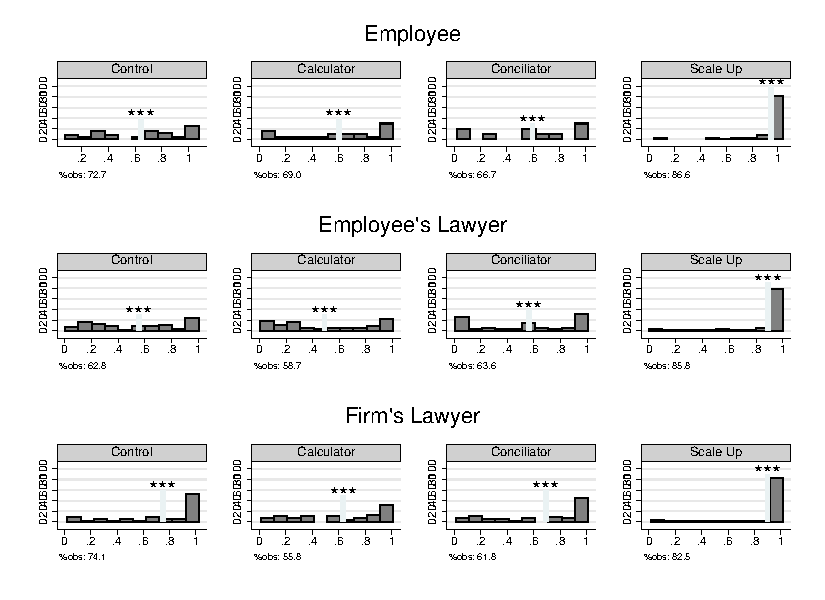
\includegraphics[width=0.70\textwidth]{updatebeleif_amount.pdf}
%\end{figure}

\end{frame}


% Placing a * after \section means it will not show in the
% outline or table of contents.
\section*{Summary}

\begin{frame}{Summary: Evidence suggestive of Private lawyer Moral hazard}
  \begin{itemize}
  \item \alert{Context:} Lawyers much more informed than workers, hard to build lawyer reputation, incentives misaligned (fixed fee for suing).
    \vspace{0.05in}
  \item \alert{Inflation of initial claim:} Private lawyers ask for much more in initial suit, conditioning for observables. But end up getting much less than asked. 
    \vspace{0.05in}
  \item  The Calculator (and conciliator) increases settlement rates, but \alert{only when worker present}.
    \vspace{0.05in}
  \item Work in progress:
  \vspace{0.05in}
    \begin{itemize}
    \item \alert{Manipulate selection of lawyer} to test whether private lawyers indeed settle less and inflate expectations
      \vspace{0.05in}
    \item Measure expectations better and include conciliated cases
      \vspace{0.05in}
    \item Robustness of calculator: how different are open vs closed cases
      \vspace{0.05in}
    \item Employee presence is endogenous: we tried to induce it by invitation but low take up
      \vspace{0.05in}
    \item Model: still undecided if we want to model lawyer moral hazard or just bargaining between worker and firm with asymmetric information
      \vspace{0.05in} 

    \end{itemize}
    
  \item  \alert{The experiment suggest ``compulsory'' conciliation may work, especially if done before lawyers get involved.}
  \end{itemize}

\end{frame}

\begin{frame}[allowframebreaks]
        \frametitle{References}
    %\nocitep{*}

\bibliographystyle{apalike}
\bibliography{References}
%\printbibliography

\end{frame}

% All of the following is optional and typically not needed. 



\begin{frame}{Summary Statistics}{Outcomes}
  \begin{table}[H]
    \label{Sum_Stats_outcomes}
    \begin{center}
       \tiny{% Table generated by Excel2LaTeX from sheet 'SS_bylawyer'
\begin{tabular}{rrrrrrr}
\toprule
Variable & Data: HD & Data: Subcourt 7 & Data: Pilot & Data: HD & Data: Subcourt 7 & Data: Pilot \\
\toprule
      & \multicolumn{3}{c}{Public Lawyer} & \multicolumn{3}{c}{Private Lawyer} \\
      \midrule
      & \multicolumn{6}{c}{Panel A: Outcomes} \\
      \midrule
      \midrule
Win   & \multicolumn{1}{l}{.66} & \multicolumn{1}{l}{.71} & \multicolumn{1}{l}{} & \multicolumn{1}{l}{.65} & \multicolumn{1}{l}{.69} & \multicolumn{1}{l}{} \\
      & \multicolumn{1}{l}{(.48)} & \multicolumn{1}{l}{(.46)} & \multicolumn{1}{l}{} & \multicolumn{1}{l}{(.48)} & \multicolumn{1}{l}{(.46)} & \multicolumn{1}{l}{} \\
Amount won & \multicolumn{1}{l}{9481} & \multicolumn{1}{l}{11093} & \multicolumn{1}{l}{} & \multicolumn{1}{l}{25532} & \multicolumn{1}{l}{22030} & \multicolumn{1}{l}{} \\
      & \multicolumn{1}{l}{(18432)} & \multicolumn{1}{l}{(24151)} & \multicolumn{1}{l}{} & \multicolumn{1}{l}{(58820)} & \multicolumn{1}{l}{(50395)} & \multicolumn{1}{l}{} \\
Total asked & \multicolumn{1}{l}{68292} & \multicolumn{1}{l}{53302} & \multicolumn{1}{l}{56045} & \multicolumn{1}{l}{373518} & \multicolumn{1}{l}{346362} & \multicolumn{1}{l}{638612} \\
      & \multicolumn{1}{l}{(241914)} & \multicolumn{1}{l}{(194606)} & \multicolumn{1}{l}{(64605)} & \multicolumn{1}{l}{(679216)} & \multicolumn{1}{l}{(581998)} & \multicolumn{1}{l}{(1462473)} \\
Win/asked & \multicolumn{1}{l}{.28} & \multicolumn{1}{l}{.38} & \multicolumn{1}{l}{} & \multicolumn{1}{l}{.2} & \multicolumn{1}{l}{.16} & \multicolumn{1}{l}{} \\
      & \multicolumn{1}{l}{(.47)} & \multicolumn{1}{l}{(.73)} & \multicolumn{1}{l}{} & \multicolumn{1}{l}{(.59)} & \multicolumn{1}{l}{(.26)} & \multicolumn{1}{l}{} \\
Conciliation  & \multicolumn{1}{l}{.64} & \multicolumn{1}{l}{.69} & \multicolumn{1}{l}{.25} & \multicolumn{1}{l}{.63} & \multicolumn{1}{l}{.67} & \multicolumn{1}{l}{.25} \\
      & \multicolumn{1}{l}{(.48)} & \multicolumn{1}{l}{(.47)} & \multicolumn{1}{l}{(.44)} & \multicolumn{1}{l}{(.48)} & \multicolumn{1}{l}{(.47)} & \multicolumn{1}{l}{(.44)} \\
Expiry & \multicolumn{1}{l}{.09} & \multicolumn{1}{l}{.04} & \multicolumn{1}{l}{} & \multicolumn{1}{l}{.08} & \multicolumn{1}{l}{.04} & \multicolumn{1}{l}{} \\
      & \multicolumn{1}{l}{(.28)} & \multicolumn{1}{l}{(.19)} & \multicolumn{1}{l}{} & \multicolumn{1}{l}{(.26)} & \multicolumn{1}{l}{(.19)} & \multicolumn{1}{l}{} \\
Drop  & \multicolumn{1}{l}{.2} & \multicolumn{1}{l}{.26} & \multicolumn{1}{l}{} & \multicolumn{1}{l}{.2} & \multicolumn{1}{l}{.26} & \multicolumn{1}{l}{} \\
      & \multicolumn{1}{l}{(.4)} & \multicolumn{1}{l}{(.44)} & \multicolumn{1}{l}{} & \multicolumn{1}{l}{(.4)} & \multicolumn{1}{l}{(.44)} & \multicolumn{1}{l}{} \\
Court/no recovery & \multicolumn{1}{l}{.06} & \multicolumn{1}{l}{0} & \multicolumn{1}{l}{} & \multicolumn{1}{l}{.07} & \multicolumn{1}{l}{.01} & \multicolumn{1}{l}{} \\
      & \multicolumn{1}{l}{(.23)} & \multicolumn{1}{l}{(0)} & \multicolumn{1}{l}{} & \multicolumn{1}{l}{(.25)} & \multicolumn{1}{l}{(.11)} & \multicolumn{1}{l}{} \\
Court/ pos recovery & \multicolumn{1}{l}{.01} & \multicolumn{1}{l}{.02} & \multicolumn{1}{l}{} & \multicolumn{1}{l}{.02} & \multicolumn{1}{l}{.02} & \multicolumn{1}{l}{} \\
      & \multicolumn{1}{l}{(.11)} & \multicolumn{1}{l}{(.12)} & \multicolumn{1}{l}{} & \multicolumn{1}{l}{(.15)} & \multicolumn{1}{l}{(.12)} & \multicolumn{1}{l}{} \\
Conciliation 1 month later & \multicolumn{1}{l}{.01} & \multicolumn{1}{l}{.01} & \multicolumn{1}{l}{0} & \multicolumn{1}{l}{.01} & \multicolumn{1}{l}{.01} & \multicolumn{1}{l}{0} \\
      & \multicolumn{1}{l}{(.11)} & \multicolumn{1}{l}{(.09)} & \multicolumn{1}{l}{(0)} & \multicolumn{1}{l}{(.09)} & \multicolumn{1}{l}{(.07)} & \multicolumn{1}{l}{(.05)} \\
Conciliation 6 month later & \multicolumn{1}{l}{.26} & \multicolumn{1}{l}{.14} & \multicolumn{1}{l}{.06} & \multicolumn{1}{l}{.28} & \multicolumn{1}{l}{.19} & \multicolumn{1}{l}{.04} \\
      & \multicolumn{1}{l}{(.44)} & \multicolumn{1}{l}{(.35)} & \multicolumn{1}{l}{(.24)} & \multicolumn{1}{l}{(.45)} & \multicolumn{1}{l}{(.39)} & \multicolumn{1}{l}{(.2)} \\
Duration & \multicolumn{1}{l}{1} & \multicolumn{1}{l}{1.04} & \multicolumn{1}{l}{} & \multicolumn{1}{l}{1.02} & \multicolumn{1}{l}{.97} & \multicolumn{1}{l}{} \\
      & \multicolumn{1}{l}{(.82)} & \multicolumn{1}{l}{(.66)} & \multicolumn{1}{l}{} & \multicolumn{1}{l}{(.97)} & \multicolumn{1}{l}{(.72)} & \multicolumn{1}{l}{} \\
      \bottomrule
\multicolumn{1}{l}{Observations} & \multicolumn{1}{l}{498} & \multicolumn{1}{l}{131} & \multicolumn{1}{l}{84} & \multicolumn{1}{l}{4497} & \multicolumn{1}{l}{725} & \multicolumn{1}{l}{730} \\
\bottomrule
\bottomrule
\end{tabular}%
}
    \end{center}
\end{table}
\end{frame}

\begin{frame}{Summary Statistics}{Basic Variables}
  \begin{table}[H]
    \label{Sum_Stats_basic_variables}
    \begin{center}https://www.sharelatex.com/project/590a73bd3ba686682a37fa2a
       \tiny{% Table generated by Excel2LaTeX from sheet 'SS_bylawyer'
\begin{tabular}{rrrrrrr}
\toprule
Variable & Data: HD & Data: Subcourt 7 & Data: Pilot & Data: HD & Data: Subcourt 7 & Data: Pilot \\
\toprule
      & \multicolumn{3}{c}{Public Lawyer} & \multicolumn{3}{c}{Private Lawyer} \\
      \midrule
      \midrule
Female & \multicolumn{1}{l}{.44} & \multicolumn{1}{l}{.33} & \multicolumn{1}{l}{.46} & \multicolumn{1}{l}{.49} & \multicolumn{1}{l}{.36} & \multicolumn{1}{l}{.4} \\
      & \multicolumn{1}{l}{(.5)} & \multicolumn{1}{l}{(.47)} & \multicolumn{1}{l}{(.5)} & \multicolumn{1}{l}{(.5)} & \multicolumn{1}{l}{(.48)} & \multicolumn{1}{l}{(.49)} \\
At will worker & \multicolumn{1}{l}{.04} & \multicolumn{1}{l}{.02} & \multicolumn{1}{l}{.1} & \multicolumn{1}{l}{.07} & \multicolumn{1}{l}{.06} & \multicolumn{1}{l}{.12} \\
      & \multicolumn{1}{l}{(.2)} & \multicolumn{1}{l}{(.15)} & \multicolumn{1}{l}{(.3)} & \multicolumn{1}{l}{(.26)} & \multicolumn{1}{l}{(.24)} & \multicolumn{1}{l}{(.33)} \\
Tenure & \multicolumn{1}{l}{2.71} & \multicolumn{1}{l}{2.81} & \multicolumn{1}{l}{2.74} & \multicolumn{1}{l}{4.33} & \multicolumn{1}{l}{3.89} & \multicolumn{1}{l}{4.96} \\
      & \multicolumn{1}{l}{(3.7)} & \multicolumn{1}{l}{(4)} & \multicolumn{1}{l}{(4.13)} & \multicolumn{1}{l}{(5.09)} & \multicolumn{1}{l}{(4.82)} & \multicolumn{1}{l}{(6.29)} \\
Daily wage & \multicolumn{1}{l}{209.5} & \multicolumn{1}{l}{229.41} & \multicolumn{1}{l}{323.12} & \multicolumn{1}{l}{498.58} & \multicolumn{1}{l}{496.29} & \multicolumn{1}{l}{863.73} \\
      & \multicolumn{1}{l}{(166.93)} & \multicolumn{1}{l}{(225.7)} & \multicolumn{1}{l}{(262.1)} & \multicolumn{1}{l}{(1155.55)} & \multicolumn{1}{l}{(698.85)} & \multicolumn{1}{l}{(1892.44)} \\
Weekly hours & \multicolumn{1}{l}{53.92} & \multicolumn{1}{l}{53.34} & \multicolumn{1}{l}{51.6} & \multicolumn{1}{l}{57.72} & \multicolumn{1}{l}{58.09} & \multicolumn{1}{l}{58.24} \\
      & \multicolumn{1}{l}{(16.69)} & \multicolumn{1}{l}{(16.19)} & \multicolumn{1}{l}{(14.28)} & \multicolumn{1}{l}{(15.28)} & \multicolumn{1}{l}{(15.36)} & \multicolumn{1}{l}{(17.16)} \\
      \midrule
      & \multicolumn{6}{c}{Panel C: Strategic variables} \\
      \midrule
      \midrule
Reinstatement & \multicolumn{1}{l}{.03} & \multicolumn{1}{l}{.02} & \multicolumn{1}{l}{.02} & .32   & .3    & \multicolumn{1}{l}{.47} \\
      & \multicolumn{1}{l}{(.16)} & \multicolumn{1}{l}{(.12)} & \multicolumn{1}{l}{(.15)} & (.47) & (.46) & \multicolumn{1}{l}{(.5)} \\
Overtime & \multicolumn{1}{l}{.18} & \multicolumn{1}{l}{.08} & \multicolumn{1}{l}{.07} & .76   & .79   & \multicolumn{1}{l}{.77} \\
      & \multicolumn{1}{l}{(.39)} & \multicolumn{1}{l}{(.28)} & \multicolumn{1}{l}{(.26)} & (.42) & (.41) & \multicolumn{1}{l}{(.43)} \\
Compulsory rest & \multicolumn{1}{l}{.09} & \multicolumn{1}{l}{.02} & \multicolumn{1}{l}{.01} & .32   & .36   & \multicolumn{1}{l}{.34} \\
      & \multicolumn{1}{l}{(.28)} & \multicolumn{1}{l}{(.12)} & \multicolumn{1}{l}{(.11)} & (.46) & (.48) & \multicolumn{1}{l}{(.47)} \\
SARIMSS & \multicolumn{1}{l}{.13} & \multicolumn{1}{l}{.05} & \multicolumn{1}{l}{.17} & .6    & .59   & \multicolumn{1}{l}{.58} \\
      & \multicolumn{1}{l}{(.34)} & \multicolumn{1}{l}{(.23)} & \multicolumn{1}{l}{(.37)} & (.49) & (.49) & \multicolumn{1}{l}{(.49)} \\
Profit sharing & \multicolumn{1}{l}{0} & \multicolumn{1}{l}{0} & \multicolumn{1}{l}{.01} & .41   & .4    & \multicolumn{1}{l}{.4} \\
      & \multicolumn{1}{l}{(.06)} & \multicolumn{1}{l}{(0)} & \multicolumn{1}{l}{(.11)} & (.49) & (.49) & \multicolumn{1}{l}{(.49)} \\
Nullification of documents & \multicolumn{1}{l}{.8} & \multicolumn{1}{l}{.76} & \multicolumn{1}{l}{.86} & .5    & .51   & \multicolumn{1}{l}{.55} \\
      & \multicolumn{1}{l}{(.4)} & \multicolumn{1}{l}{(.43)} & \multicolumn{1}{l}{(.35)} & (.5)  & (.5)  & \multicolumn{1}{l}{(.5)} \\
Co-defendant & \multicolumn{1}{l}{.03} & \multicolumn{1}{l}{.02} & \multicolumn{1}{l}{.07} & .13   & .12   & \multicolumn{1}{l}{.11} \\
      & \multicolumn{1}{l}{(.17)} & \multicolumn{1}{l}{(.12)} & \multicolumn{1}{l}{(.26)} & (.34) & (.33) & \multicolumn{1}{l}{(.31)} \\
      \bottomrule
\multicolumn{1}{l}{Observations} & \multicolumn{1}{l}{498} & \multicolumn{1}{l}{131} & \multicolumn{1}{l}{84} & \multicolumn{1}{l}{4497} & \multicolumn{1}{l}{725} & \multicolumn{1}{l}{730} \\
\bottomrule
\bottomrule
\end{tabular}%
}
    \end{center}
\end{table}
\end{frame}

\begin{frame}{Summary Statistics}{Strategic variables}
  \begin{table}[H]
    \label{Sum_Stats_strategic_variables}
    \begin{center}
       \tiny{% Table generated by Excel2LaTeX from sheet 'SS_bylawyer'
\begin{tabular}{rrrrrrr}
\toprule
Variable & Data: HD & Data: Subcourt 7 & Data: Pilot & Data: HD & Data: Subcourt 7 & Data: Pilot \\
\toprule
      & \multicolumn{3}{c}{Public Lawyer} & \multicolumn{3}{c}{Private Lawyer} \\
      \midrule
      \midrule
Reinstatement & \multicolumn{1}{l}{.03} & \multicolumn{1}{l}{.02} & \multicolumn{1}{l}{.02} & .32   & .3    & \multicolumn{1}{l}{.47} \\
      & \multicolumn{1}{l}{(.16)} & \multicolumn{1}{l}{(.12)} & \multicolumn{1}{l}{(.15)} & (.47) & (.46) & \multicolumn{1}{l}{(.5)} \\
Overtime & \multicolumn{1}{l}{.18} & \multicolumn{1}{l}{.08} & \multicolumn{1}{l}{.07} & .76   & .79   & \multicolumn{1}{l}{.77} \\
      & \multicolumn{1}{l}{(.39)} & \multicolumn{1}{l}{(.28)} & \multicolumn{1}{l}{(.26)} & (.42) & (.41) & \multicolumn{1}{l}{(.43)} \\
Compulsory rest & \multicolumn{1}{l}{.09} & \multicolumn{1}{l}{.02} & \multicolumn{1}{l}{.01} & .32   & .36   & \multicolumn{1}{l}{.34} \\
      & \multicolumn{1}{l}{(.28)} & \multicolumn{1}{l}{(.12)} & \multicolumn{1}{l}{(.11)} & (.46) & (.48) & \multicolumn{1}{l}{(.47)} \\
SARIMSS & \multicolumn{1}{l}{.13} & \multicolumn{1}{l}{.05} & \multicolumn{1}{l}{.17} & .6    & .59   & \multicolumn{1}{l}{.58} \\
      & \multicolumn{1}{l}{(.34)} & \multicolumn{1}{l}{(.23)} & \multicolumn{1}{l}{(.37)} & (.49) & (.49) & \multicolumn{1}{l}{(.49)} \\
Profit sharing & \multicolumn{1}{l}{0} & \multicolumn{1}{l}{0} & \multicolumn{1}{l}{.01} & .41   & .4    & \multicolumn{1}{l}{.4} \\
      & \multicolumn{1}{l}{(.06)} & \multicolumn{1}{l}{(0)} & \multicolumn{1}{l}{(.11)} & (.49) & (.49) & \multicolumn{1}{l}{(.49)} \\
Nullification of documents & \multicolumn{1}{l}{.8} & \multicolumn{1}{l}{.76} & \multicolumn{1}{l}{.86} & .5    & .51   & \multicolumn{1}{l}{.55} \\
      & \multicolumn{1}{l}{(.4)} & \multicolumn{1}{l}{(.43)} & \multicolumn{1}{l}{(.35)} & (.5)  & (.5)  & \multicolumn{1}{l}{(.5)} \\
Co-defendant & \multicolumn{1}{l}{.03} & \multicolumn{1}{l}{.02} & \multicolumn{1}{l}{.07} & .13   & .12   & \multicolumn{1}{l}{.11} \\
      & \multicolumn{1}{l}{(.17)} & \multicolumn{1}{l}{(.12)} & \multicolumn{1}{l}{(.26)} & (.34) & (.33) & \multicolumn{1}{l}{(.31)} \\
      \bottomrule
\multicolumn{1}{l}{Observations} & \multicolumn{1}{l}{498} & \multicolumn{1}{l}{131} & \multicolumn{1}{l}{84} & \multicolumn{1}{l}{4497} & \multicolumn{1}{l}{725} & \multicolumn{1}{l}{730} \\
\bottomrule
\bottomrule
\end{tabular}%
}
    \end{center}
\end{table}
\end{frame}

\begin{frame}{Baseline Expectations}
\begin{table}[H]
    \label{Table_expectations}
    \begin{center}
       \scriptsize{% Table generated by Excel2LaTeX from sheet 'SS_A'
\begin{tabular}{rrrr}
\toprule
      & \multicolumn{1}{c}{Total} & \multicolumn{1}{c}{Public Lawyer} & \multicolumn{1}{c}{Private Lawyer} \\
\midrule
\multicolumn{1}{l}{Variable} & \multicolumn{3}{c}{Employee} \\
\midrule
\midrule
\multicolumn{1}{l}{Prob winning} & \multicolumn{1}{l}{.8} & \multicolumn{1}{l}{.79} & \multicolumn{1}{l}{.8} \\
\multicolumn{1}{l}{} & \multicolumn{1}{l}{(.23)} & \multicolumn{1}{l}{(.23)} & \multicolumn{1}{l}{(.23)} \\
\multicolumn{1}{l}{Most prob amount} & \multicolumn{1}{l}{75478.14} & \multicolumn{1}{l}{37543.06} & \multicolumn{1}{l}{89134.77} \\
\multicolumn{1}{l}{} & \multicolumn{1}{l}{(263891)} & \multicolumn{1}{l}{(54321.51)} & \multicolumn{1}{l}{(305297.61)} \\
\multicolumn{1}{l}{Most prob duration} & \multicolumn{1}{l}{2.68} & \multicolumn{1}{l}{2.58} & \multicolumn{1}{l}{2.72} \\
\multicolumn{1}{l}{} & \multicolumn{1}{l}{(1.74)} & \multicolumn{1}{l}{(1.97)} & \multicolumn{1}{l}{(1.65)} \\
\multicolumn{1}{l}{Obs} & \multicolumn{1}{l}{136} & \multicolumn{1}{l}{36} & \multicolumn{1}{l}{98} \\
\midrule
\multicolumn{1}{l}{} & \multicolumn{3}{c}{Employee's Lawyer} \\
\midrule
\midrule
\multicolumn{1}{l}{Prob winning} & \multicolumn{1}{l}{.73} & \multicolumn{1}{l}{.62} & \multicolumn{1}{l}{.74} \\
\multicolumn{1}{l}{} & \multicolumn{1}{l}{(.2)} & \multicolumn{1}{l}{(.19)} & \multicolumn{1}{l}{(.2)} \\
\multicolumn{1}{l}{Most prob amount} & \multicolumn{1}{l}{214904.55} & \multicolumn{1}{l}{38127} & \multicolumn{1}{l}{233710.68} \\
\multicolumn{1}{l}{} & \multicolumn{1}{l}{(1291234.24)} & \multicolumn{1}{l}{(81074.83)} & \multicolumn{1}{l}{(1356804.44)} \\
\multicolumn{1}{l}{Most prob duration} & \multicolumn{1}{l}{3.67} & \multicolumn{1}{l}{5.41} & \multicolumn{1}{l}{3.48} \\
\multicolumn{1}{l}{} & \multicolumn{1}{l}{(1.9)} & \multicolumn{1}{l}{(2.35)} & \multicolumn{1}{l}{(1.75)} \\
\multicolumn{1}{l}{Obs} & \multicolumn{1}{l}{312} & \multicolumn{1}{l}{30} & \multicolumn{1}{l}{282} \\
\midrule
\multicolumn{1}{l}{} & \multicolumn{3}{c}{Firm's Lawyer} \\
\midrule
\midrule
\multicolumn{1}{l}{Prob winning} & \multicolumn{1}{l}{0.68} & \multicolumn{1}{l}{.74} & \multicolumn{1}{l}{.67} \\
\multicolumn{1}{l}{} & \multicolumn{1}{l}{(.22)} & \multicolumn{1}{l}{(.22)} & \multicolumn{1}{l}{(.22)} \\
\multicolumn{1}{l}{Most prob amount} & \multicolumn{1}{l}{58052.43} & \multicolumn{1}{l}{13035.84} & \multicolumn{1}{l}{62539.61} \\
\multicolumn{1}{l}{} & \multicolumn{1}{l}{(239962.38)} & \multicolumn{1}{l}{(15724.8)} & \multicolumn{1}{l}{(251183.91)} \\
\multicolumn{1}{l}{Most prob duration} & \multicolumn{1}{l}{4.07} & \multicolumn{1}{l}{3.45} & \multicolumn{1}{l}{4.13} \\
\multicolumn{1}{l}{} & \multicolumn{1}{l}{(2.11)} & \multicolumn{1}{l}{(1.67)} & \multicolumn{1}{l}{(2.14)} \\
\multicolumn{1}{l}{Obs} & \multicolumn{1}{l}{342} & \multicolumn{1}{l}{31} & \multicolumn{1}{l}{311} \\
\bottomrule
\bottomrule
\end{tabular}%
}
    \end{center}
\end{table}
    \footnotesize    
    \textit{Notes:} 
    Summary statistics of parties' beliefs. We show mean and standard deviation for the whole sample, \& dividing by type of employee's lawyer.
\end{frame}



\begin{frame}{Compliance rate}
 \begin{table}[H]
  \resizebox{0.9\textwidth}{!}{\begin{minipage}{\textwidth}
\label{Table_compliance}
\begin{center}
\scriptsize{% Table generated by Excel2LaTeX from sheet 'Compliance'
\begin{tabular}{lrccc}
\toprule
      & \multicolumn{1}{c}{(1)} & (2)   & (3)   & (4) \\
\midrule
      & \multicolumn{1}{c}{Treatment assignment} & Compliance with treatment & Compliance Baseline survey & Compliance Exit survey \\
\midrule
\midrule
Control & 1994  & -     & 0.40  & 0.45 \\
Calculadora  & 364   & 78.02 & 75.27 & 56.87 \\
Conciliadora & 351   & 72.08 & 68.95 & 54.42 \\
\bottomrule
\end{tabular}%
}
\end{center}
\end{minipage}}
\end{table}
 \footnotesize
\textit{Notes:} 
The number of cases assigned to the 3 different groups is very similar, and is close to 7 per day on average. The compliance with treatment rate is similar for both treatments and in the range of 75\%.
\end{frame}



\begin{frame}{Conciliation over time}
    \begin{figure}[H]
    \label{Figure_dynamicsConciliation}
    \begin{center}
        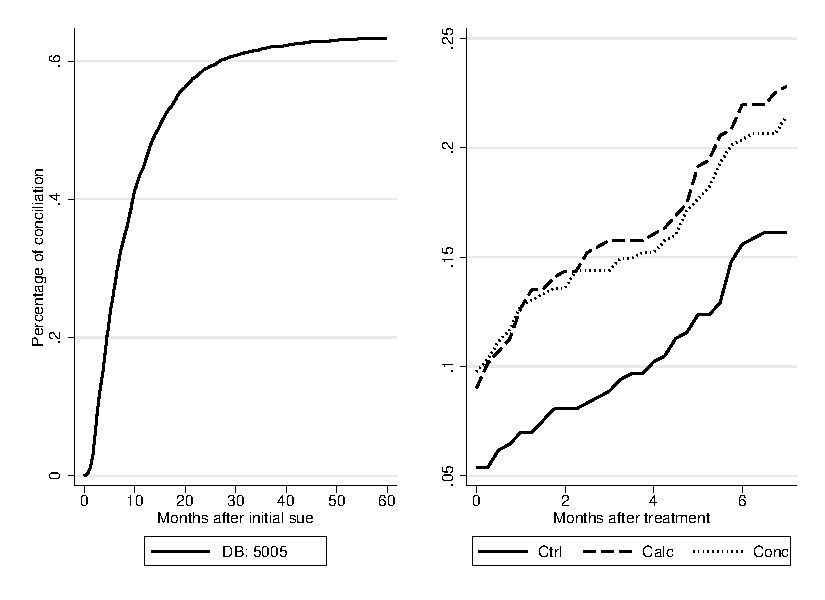
\includegraphics[width=0.7\textwidth]{con_overtime.pdf}
        \end{center}
        {\footnotesize \textit{Notes: } Conciliation over time in HD database and pilot database.}
\end{figure}
\end{frame}



\end{document}


